\documentclass{beamer}
\usepackage{beamerfoils}
\usepackage[latin9]{inputenc}
\usepackage{ngerman}

\newcommand\emptyline{\\\ \\}

\title{Einf�hrung in BibSonomy2}
\author{Jens Illig und Christian Schenk}
\date{19. September 2007}

\begin{document}
\maketitle


\foilhead{Agenda}
\begin{enumerate}
\item Motivation
\item REST
\item Maven
\item iBatis
\item Spring
\item Eclipse
\item �berblick
\end{enumerate}


\foilhead{Motivation}
Warum ein \emph{neues} BibSonomy?\emptyline

Weil:
\begin{enumerate}
\item Bereitstellen der vorhandenen Features als Webservice (REST-API)
\item Aufr�umen des Codes
\end{enumerate}


\foilhead{REST: Was ist das?}
\begin{itemize}
	\item kein Standard
	\item 2000 in Dissertation von Roy Thomas Fielding beschrieben
	\item ein Architekturstil (koordinierte Menge von Architekturconstraints)
	\item \emph{\dq architectural model for how the web should work\dq}
	\item Grundlage alternativer Web Service Systeme
\end{itemize}

\foilhead{REST $\leftrightarrow$ Web Service ?}
\begin{itemize}
	\item oft: maschinenverst\"andlich
	\item Interface zu Diensten einer Applikation
	\item Web-Technologien (HTTP,URI,XML)
	\item SOAP (XML-Nachrichtenrahmen und RPC-Protokollformat)
	\item WSDL (Beschreibung von SOAP Diensten)
	\item REST (wann ist ein Web Service wirklich Teil des Webs?)
\end{itemize}

\foilhead{REST $\leftrightarrow$ Web ?}
\begin{itemize}
	\item RESTful
		\begin{itemize}
			\item HTTP $\Rightarrow$ Client-Server, Stateless, Cache, Selbstbeschreibende Anfragen
			\item URI $\Rightarrow$ Eindeutige Identifikation von Ressourcen
			\item (X)HTML $\Rightarrow$ Hypermedia als Beschreibung des Applikationsstatus
			\item CGI... $\Rightarrow$ Layered System, Manipulation von Ressourcen durch Repr\"asentationen
		\end{itemize}
	\item RESTless
		\begin{itemize}
			\item Session-Tracking $\Rightarrow$ keine eindeutige Identifikation von Ressourcen
			\item Cookies $\Rightarrow$ keine selbstbeschreibenden Anfragen
			\item Frames $\Rightarrow$ Probleme bei Hypermedia als Beschreibung des Applikationsstatus
		\end{itemize}
\end{itemize}


\foilhead{Maven}
Warum Maven?\emptyline

Es\ldots
\begin{enumerate}
\item standardisiert Projektstruktur
\item verwaltet Abh�ngigkeiten
\item erstellt Artefakte
\end{enumerate}


\foilhead{Continuum}
Warum Continuum?\emptyline

Es\ldots
\begin{enumerate}
\item verwendet Maven
\item compiled
\item startet Testcases
\item verschickt Mails
\end{enumerate}

$\Rightarrow$ erm\"oglicht konsequentes Continuous Integration


\foilhead{iBatis}
Warum iBatis?\emptyline

Es\ldots
\begin{enumerate}
\item verwaltet Datenbankkonfiguration
\item organisiert SQL-Statements
\item stellt Anfragen an die Datenbank
\end{enumerate}


\foilhead{Spring}
Warum Spring?\emptyline

Es\ldots
\begin{enumerate}
\item verlangt in Komponenten zu denken
\item erzeugt konfigurierte Komponenten zur Laufzeit
\item bietet \emph{viele Dinge} out-of-the-box
\end{enumerate}


\foilhead{Eclipse}
Warum Eclipse?\emptyline

Es\ldots
\begin{enumerate}
\item integriert die o.g. Werkzeuge
\item verwaltet Projekteinstellungen f�r jeden Entwickler einheitlich
\end{enumerate}


\foilhead{\"Uberblick: Projektmodule}
\begin{figure}[ht] \centering
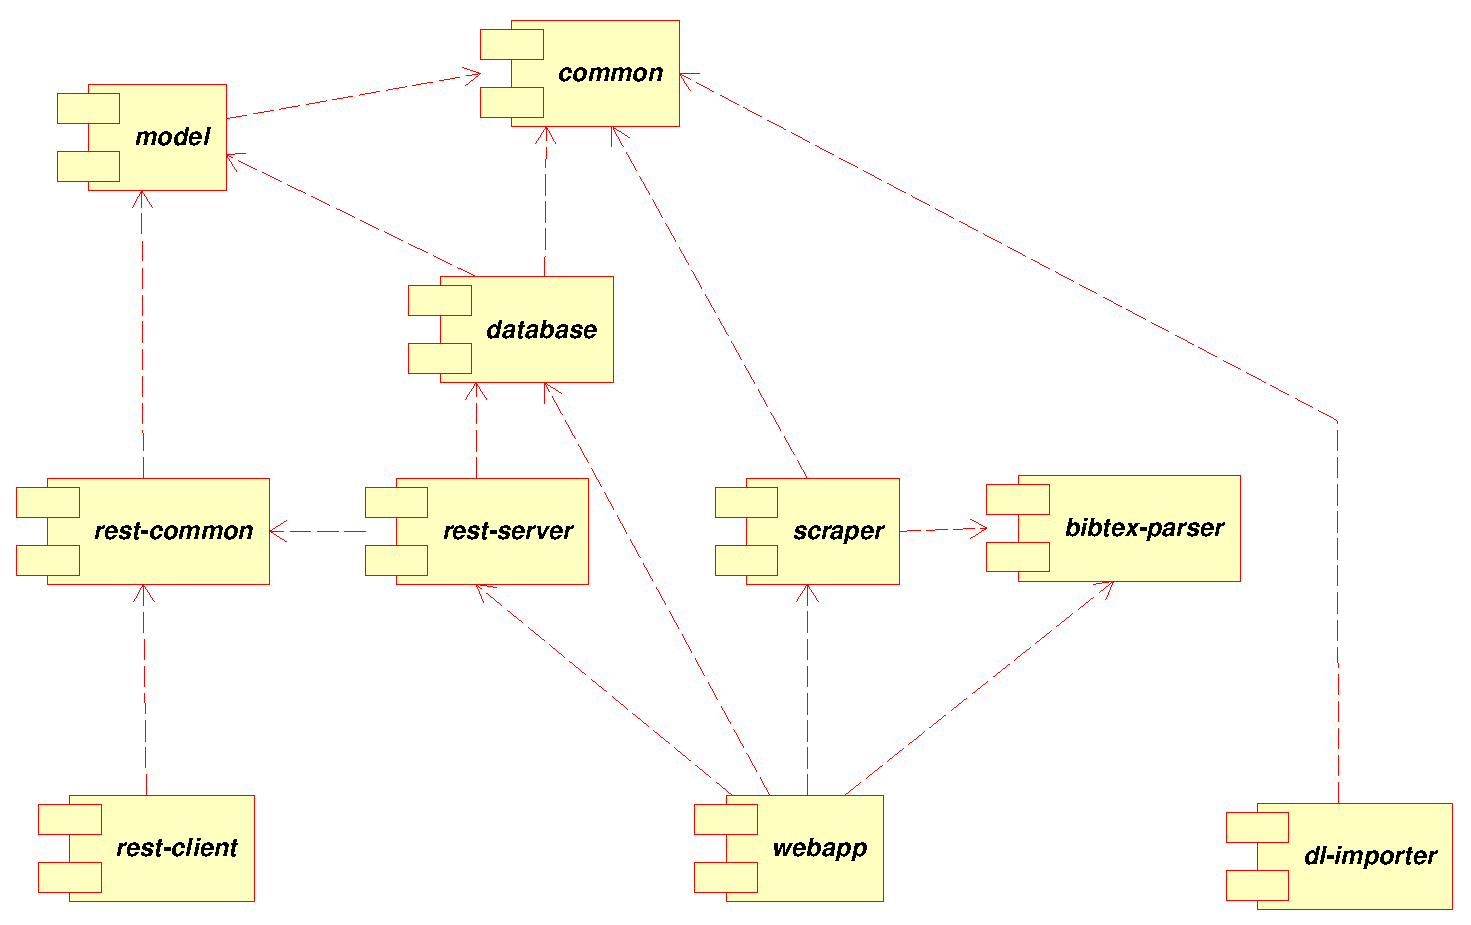
\includegraphics[width=11cm]{modules.eps}
\end{figure}

\foilhead{\"Uberblick: Datenbankabstraktion}
\begin{figure}[ht] \centering
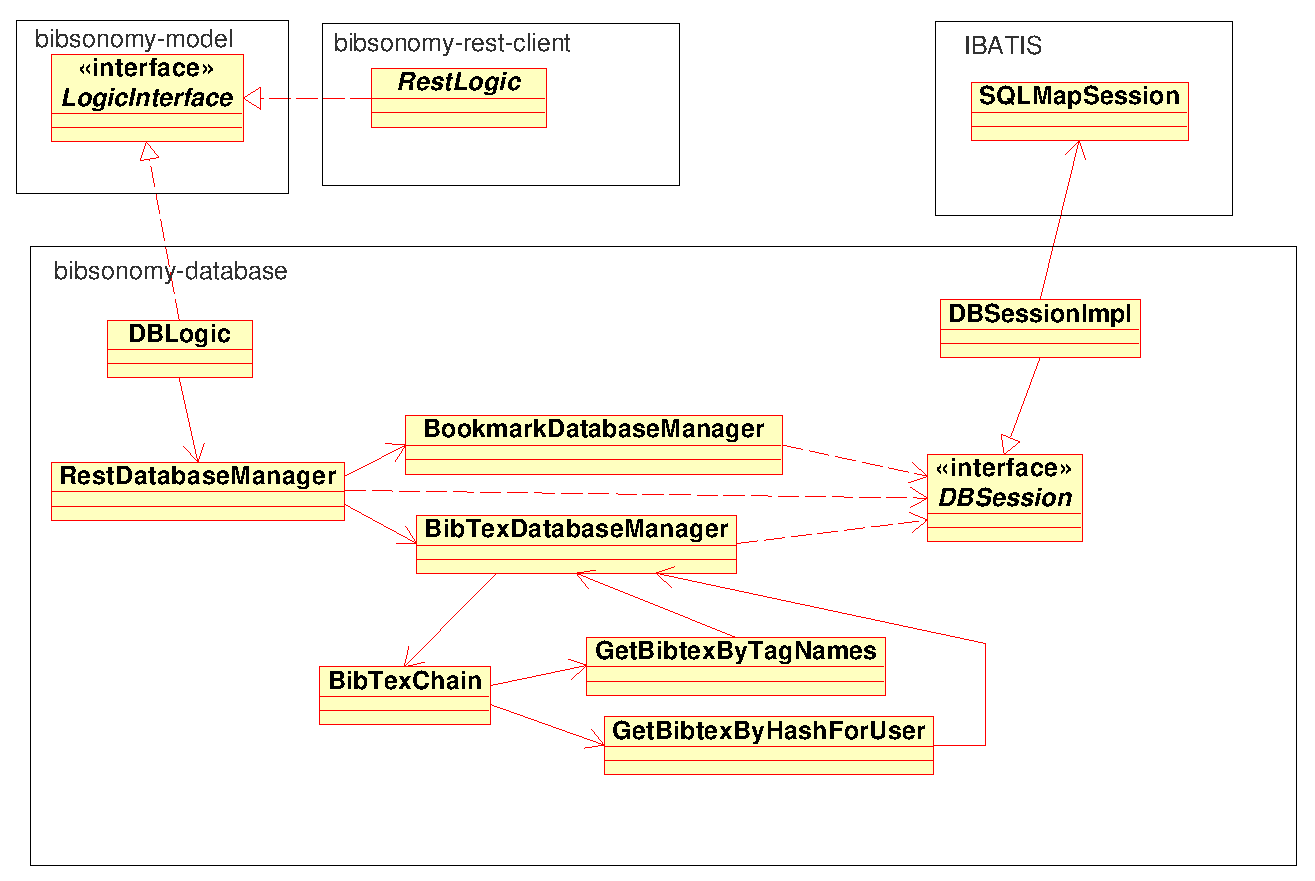
\includegraphics[width=11cm]{DB_classes.eps}
\end{figure}

\foilhead{Ende}
\begin{center}
Soweit sogut\ldots ?
\end{center}

\endfoil
\end{document}
